\documentclass[11pt]{article}
\usepackage[margin=0.75in]{geometry}
\usepackage{amsmath}
\usepackage{tikz}
\usepackage{enumitem}
\usepackage{siunitx}
\setlength{\parindent}{0pt}
\newcommand{\graphbox}{\begin{center}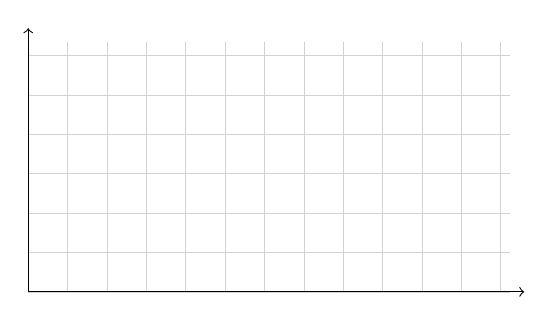
\begin{tikzpicture}[x=0.72cm,y=0.72cm]
\draw[step=0.5cm,gray!35,very thin] (0,0) grid (8.5,4.4);
\draw[->] (0,0)--(8.75,0); \draw[->] (0,0)--(0,4.65);
\end{tikzpicture}\end{center}}
\begin{document}
\begin{center}\Large\textbf{AP Physics 1 1D Motion Post-Lab Quiz -- Version E}\end{center}
\vspace{0.08in}\textbf{Name:} \rule{2.1in}{0.4pt}\hfill\textbf{Period:} \rule{0.65in}{0.4pt}\hfill\textbf{Date:} \rule{1.1in}{0.4pt}
\vspace{0.12in}
\begin{enumerate}[leftmargin=*,itemsep=0.15in]
\item A ball is released from rest from a fixed height and falls straight downward. A student wants to compare the ball's motion near the beginning, middle, and end of the fall.

\textbf{a.} Describe the measurements the student should collect.\\
\textbf{b.} Describe the pattern in those measurements that would show that the ball is speeding up.
\vspace{0.55in}

\item A student records a ball falling vertically while a meterstick is positioned vertically next to the path of the ball and is clearly visible in the video.

\textbf{a.} Explain how the student could use the video and meterstick together to determine the ball's position at several different times.\\
\textbf{b.} Explain one advantage of collecting the position and time measurements from the recording rather than trying to make the measurements while the ball is falling.
\vspace{0.55in}

\item A student drops a ball from rest and records the following measurements.

\begin{center}
\begin{tabular}{c|cccccc}
Time $t$ (s) & 0.00 & 0.10 & 0.20 & 0.30 & 0.40 & 0.50\\ \hline
Distance fallen $d$ (m) & 0.000 & 0.051 & 0.193 & 0.441 & 0.789 & 1.225
\end{tabular}
\end{center}
\textbf{a.} Transform the data as needed to produce a linear graph. Using the graph space provided, plot the appropriate variables, clearly label both axes with units, and draw a best-fit line.\\
\textbf{b.} Describe the shape of your graph. Based on the graph, determine whether the ball's acceleration was approximately constant and explain your reasoning.

\graphbox
\end{enumerate}
\end{document}
